\section{Event displays}
\label{app:event-displays}
Figure~\ref{fig:event-display-1} shows an example event display for an event which passes all analysis cuts.

\begin{figure}[h!]
  \centering
  \includegraphics[page=26,width=0.48\textwidth]{figures/EventDisplays.pdf}
  \includegraphics[page=27,width=0.48\textwidth]{figures/EventDisplays.pdf} \\
  \includegraphics[page=29,width=0.48\textwidth]{figures/EventDisplays.pdf}
  \includegraphics[page=30,width=0.48\textwidth]{figures/EventDisplays.pdf}
  \caption{Event display for an event that passes all cuts. 
    The muons are shown as red dots, the charged particles (hadrons or tracks) are shown as gray or black crosses and the dilepton system is displayed as a red cross, separately at the reconstructed level (top left) and at the particle level (top right). 
    %, the centre of the dilepton system is shown with a red X and the individual muons with a red dot.
    Track jets are shown as blue circles, and leading jet constituents are represented with black crosses.
    % while other jet constituents are shown with a purple X. 
    The leading jet is also shown (bottom left) simulaniously for reconstructed tracks and truth charged hadrons, and most particle momenta are listed (bottom right).
    %with the reconstructed constituents represented by a black X, and truth charged hadrons represented by a blue circle.}
    More event displays like this are listed in Appendix~\ref{app:event-displays}. 
    Note that the goal with this analysis is to provide unfolded events that contain a list of four vectors corresponding to all individual particles seen in the upper right figure: two muons, and a full list of charged hadrons particles.}
  \label{fig:event-display-1}
\end{figure}
